\documentclass{beamer}

\usepackage[utf8]{inputenc}
\usepackage[spanish]{babel}
%\usepackage{times}
\usepackage{graphicx}
\usepackage{amsmath}
\usepackage{amsthm}
\usepackage{amssymb} 

\theoremstyle{definition}
\newtheorem{Def}{Definición}
\newtheorem{Prop}{Proposición}

\spanishdecimal{.}


\mode<presentation> {
  \usetheme{Madrid}
  \setbeamercovered{transparent}
}

\title[] %
{¿Qué representan los subconjuntos difusos?}
\subtitle{Gradualidad, incertidumbre, vaguedad y bipolaridad}

\author[Waissman]{Julio Waissman Vilanova}

\institute[UNISON] %
{Departamento de Matem\'aticas\\
 \textbf{Universidad de Sonora}}


\subject{Fuzzy Systems}


\begin{document}


\begin{frame}
  \titlepage
\end{frame}

\begin{frame}
  \frametitle{Plan de la presentación}
  \tableofcontents
  %  % You might wish to add the option [pausesections]
\end{frame}


% Sección
\section{Conocimiento gradual}

\begin{frame}
  \frametitle{¿Que representa un conjunto?}
   \begin{block}{Georg Cantor (Wikipedia)}
      ``...entiendo en general por variedad o \alert{conjunto} toda
      multiplicidad que puede ser pensada como unidad, esto es, toda
      colección de elementos determinados que pueden ser unidos en una
      totalidad mediante una ley.''
   \end{block}
   \vspace{1cm}
   \begin{description}
   \item[Conjuntos Ónticos:] Representan un objeto  o concepto que se
     compone de la conjunción de sus elementos.
   \item[Conjuntos Epistémicos:] Conjunto de valores, de los cuales
     uno es correcto, representa un constructo.  
   \end{description}
  
\end{frame}

\begin{frame}
  \frametitle{Subconjuntos difusos}
  \begin{itemize}
  \item Sea $\Omega$ un conjunto universo
  \item A la función $A: \Omega \to [0, 1]$ se le conoce como conjunto
    difuso.
  \item $A(x)$ es la \emph{pertenencia} de $x \in U$ al subconjunto
    difuso $A$.
  \item Definir $A$ puede ser subjetivo, pero en su definición no hay
    incertidumbre. 
  \item Los subconjuntos difusos clásicos son \emph{subconjuntos
      difusos ónticos}. 
  \end{itemize}

  \begin{center}
    \alert{Los subconjuntos difusos representan la noción de
      \emph{gradualidad} en el conocimiento, debido al uso de lenguaje natural}
  \end{center}
\end{frame}

\begin{frame}
  \frametitle{Ejemplo: ¿La imagen es ``bosque''?}
\begin{center}
\only<1>{
\includegraphics[width=0.8\textwidth]{bosque1.jpg}}
\only<2>{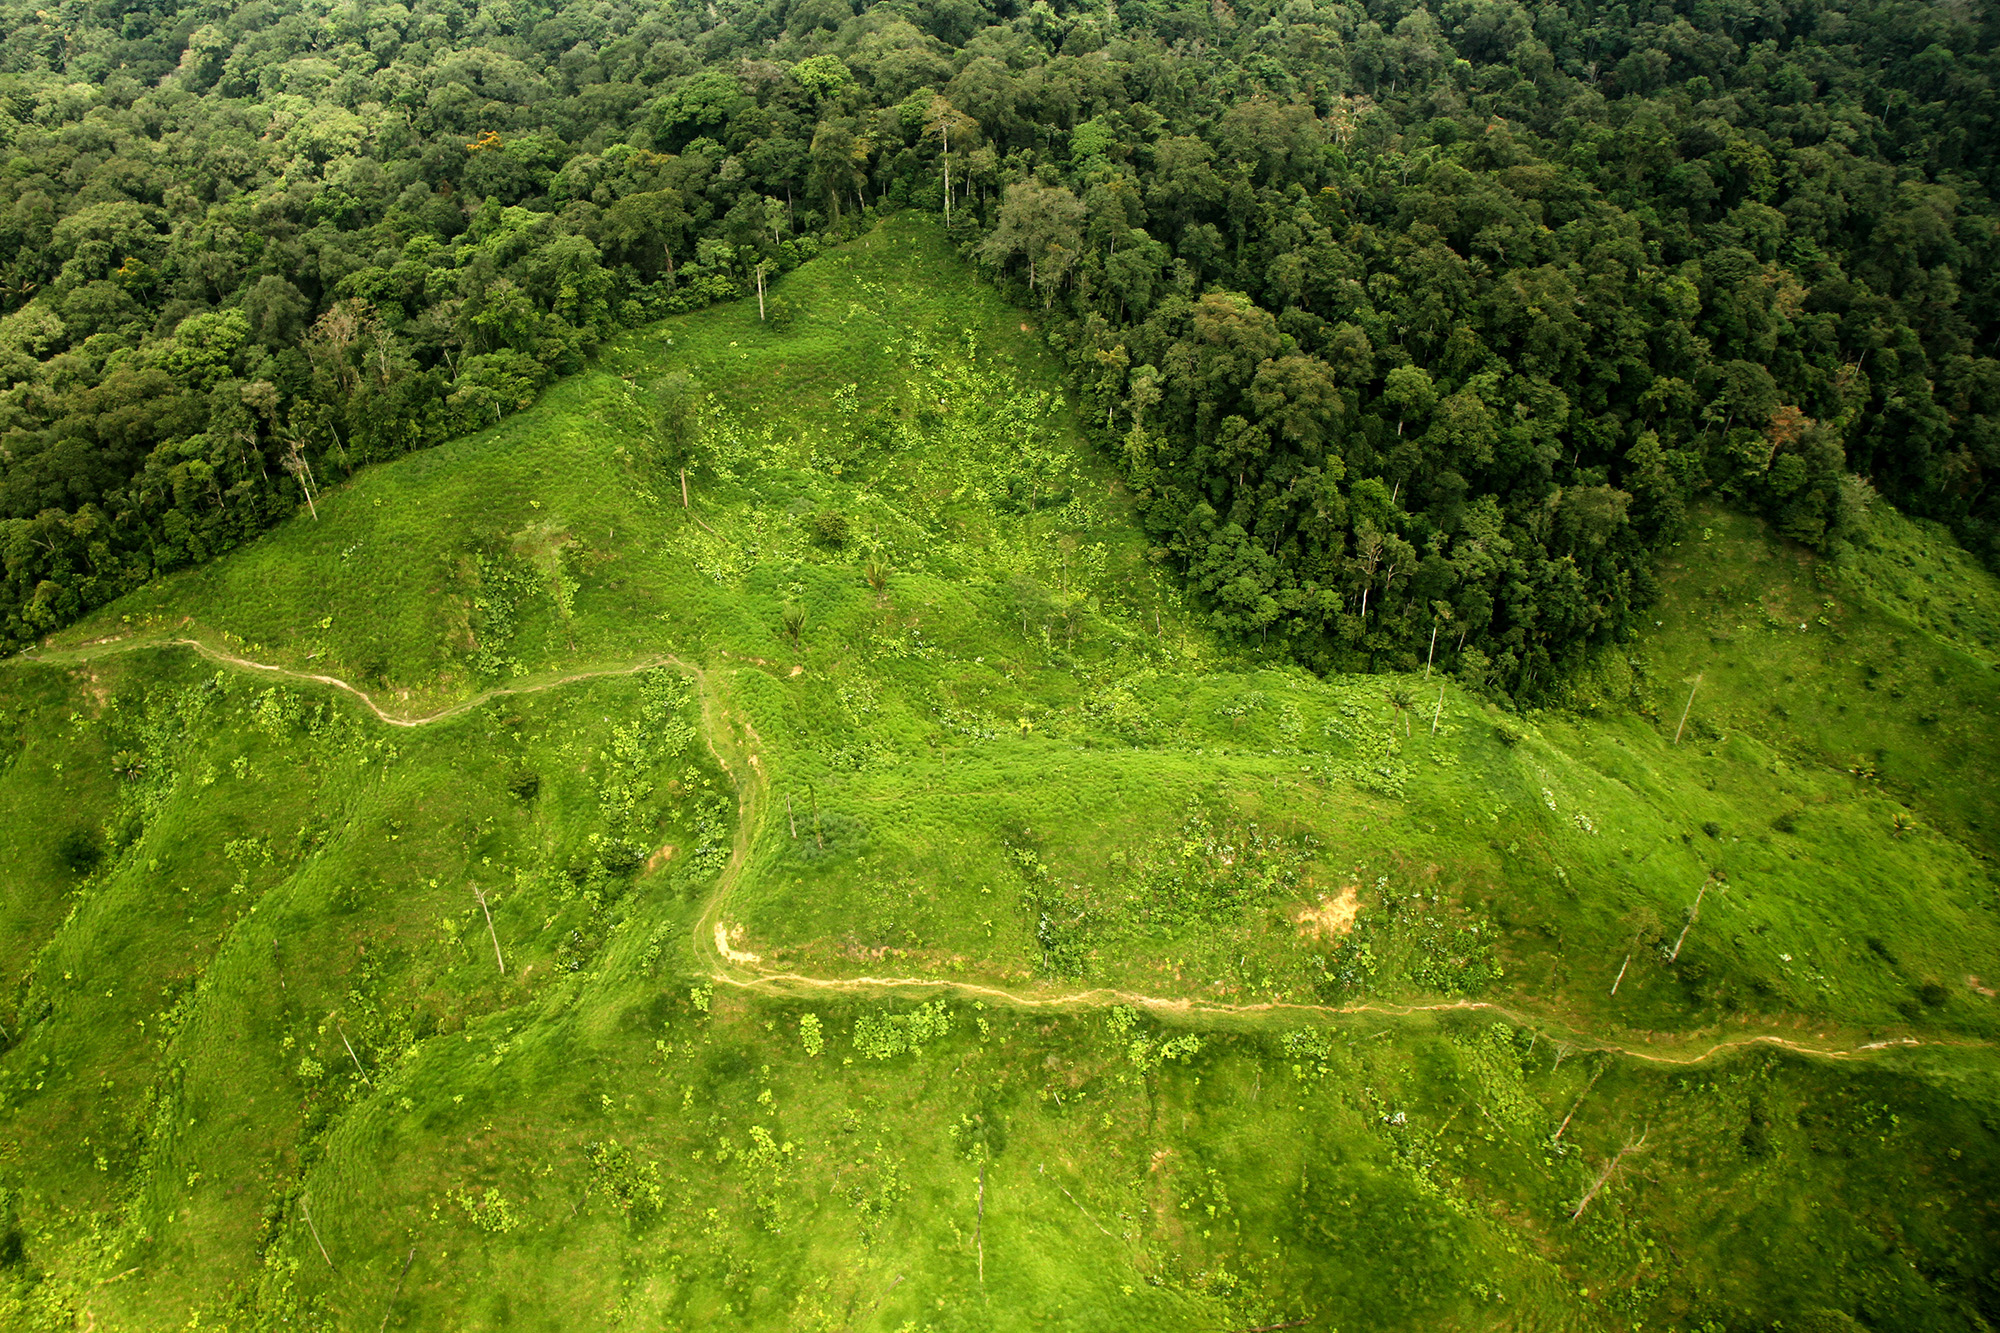
\includegraphics[width=0.8\textwidth]{bosque2.jpg}}
\only<3>{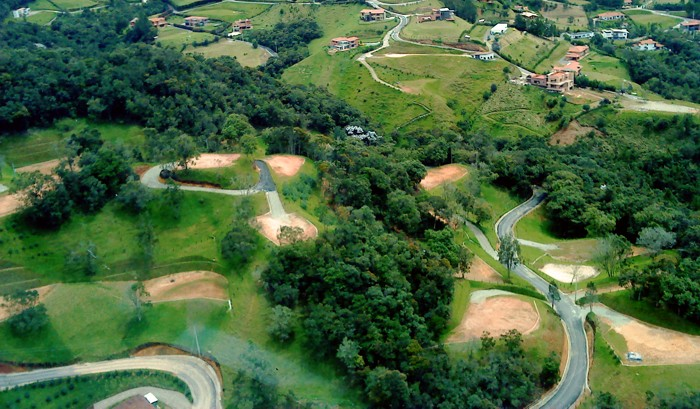
\includegraphics[width=0.8\textwidth]{bosque3.jpg}}
\only<4>{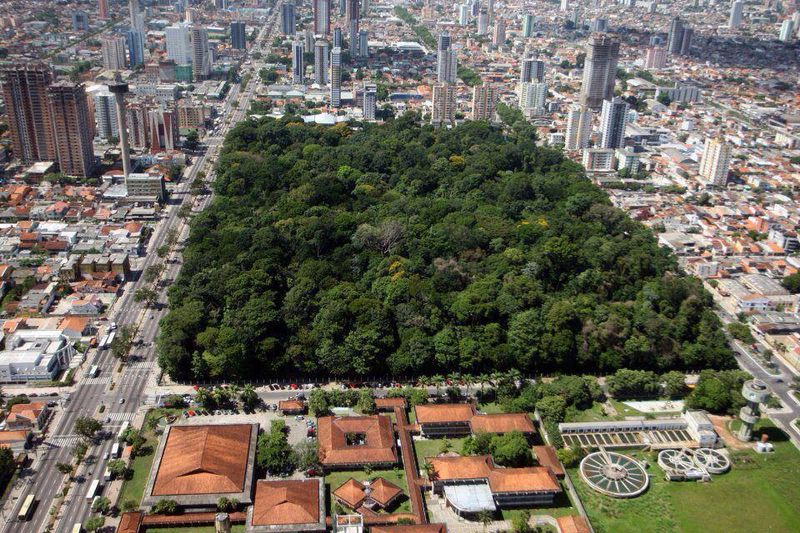
\includegraphics[width=0.8\textwidth]{bosque4.jpg}}
\only<5>{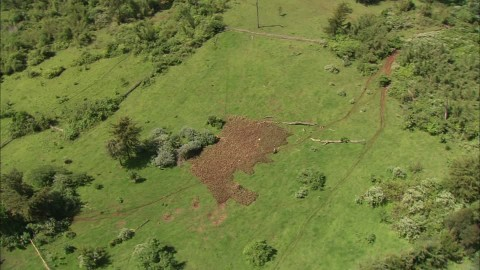
\includegraphics[width=0.8\textwidth]{bosque5.jpg}}
\only<6>{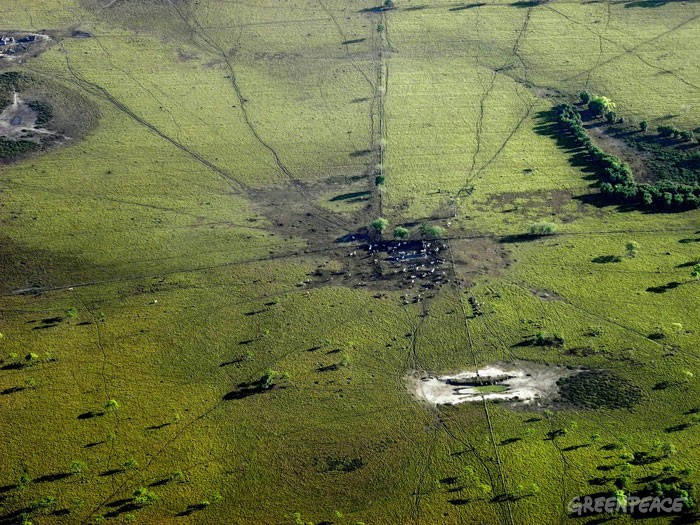
\includegraphics[width=0.8\textwidth]{bosque6.jpg}}
\end{center}  
\end{frame}

\begin{frame}
  \frametitle{Operaciones básicas}
  \begin{block}{Si $A, B : \Omega \to [0, 1]$, en términos \emph{muy} reducionistas:}
    
    \begin{itemize}
    \item $A \cap B (x) = \min(A(x), B(x))$
    \item $A \cup B (x) = \max(A(x), B(x))$
    \item $A^c(x) = 1 - A(x)$
    \end{itemize}    
  
  \end{block}
  \vspace{1cm}  
   Por lo tanto, 
   
   $$A \cap A^c (x) = \min(A(x), 1 - A(x)) \leq 0.5$$
  \end{frame}

\section{Incertidumbre}

\begin{frame}
  \frametitle{¿Existen subconjuntos difusos epistémicos?}
  \begin{block}{Distribución de posibilidad}
    Sea $\Omega$ un conjunto finito, una distribución de posibilidad es una
    función $\Pi: 2^\Omega \to [0, 1]$ tal que:
    \begin{itemize}
    \item $\Pi(\emptyset) = 0$,
    \item $\Pi(\Omega) = 1$,
    \item $\Pi(U \cup V) = \max(\Pi(U), \Pi(V))$ para $U, V \subseteq
      \Omega$, conjuntos disjuntos. 
    \end{itemize}
  \end{block}
\vspace{0.5cm}
y por lo tanto
$$
\Pi(U) = \max_{x \in U} \Pi(\{x\}),
$$
donde $\Pi(\{x\})$ puede ser la pertenencia de x a un conjunto difuso.

\vspace{0.5cm}

\textbf{Ejemplo:} En un conjunto de imágenes aéreas, ¿Cuál es la posibilidad
de encontrar ``bosque''?

\end{frame}

\section{Vaguedad}

\begin{frame}
  \frametitle{Vaguedad: un ejemplo en lógica de predicados}
Consideremos un conjunto de 5 predicados $\{p_1, p_2, p_3, p_4, p_5\}$ tal
que $t(p_i) \in \{F, V\}$.

\begin{itemize}
\item $A_* = \{p_5\}$ el conjunto de predicados que seguro $t(p_i) = T$,
\item $A^* = \{p_2, p_3, p_4, p_5\}$ el conjunto de predicados que
  podrían ser que $t(p_i)= T$.
\item Entonces, $t(p_1) = F$, $t(p_5) = T$, y $t(p_i) \in \{F, V\}$
  para $i \in \{2, 3, 4\}$.
\item $t(p_i) \in \{F, V\}$ no es otro valor de verdad. 
\item La lógica trivaluada de Kleen representaba vaguedad, mientras que la
  lógica trivaluada de Luckasiewicz representaba gradualidad. 
\end{itemize}
\end{frame}

\begin{frame}
  \frametitle{Vaguedad en subconjuntos difusos ónticos}
  Dos maneras claras de representar la vaguedad:

  \begin{description}
  \item[Subconjunto difuso tipo 2] es una función
    $\tilde{A}: \Omega \to \mathcal{F}$, donde
    $\mathcal{F} = \{f | f: [0, 1] \to [0, 1]\}$.
  \item[Subconjunto difuso evaluado en intervalo,] donde $\bar{A}(x) =
    [A_*(x), A^*(x)]$ es un intervalo
    cerrado de $[0, 1]$, donde $A_*$ y $A^*$
    son subconjuntos difusos de $\Omega$ tal que $A_*(x) \leq A^*(x)$
    para toda $x \in \Omega$. 
  \end{description}

\textbf{Utilizando aritmética de intervalos:}
  \begin{itemize}
  \item $\bar{A} \cap \bar{B} (x) = [\min(A_*(x), B_*(x)), \min(A^*(x), B^*(x))]$,
  \item $\bar{A} \cup \bar{B} (x) = [\max(A_*(x), B_*(x)), \max(A^*(x), B^*(x))]$,
  \item $\bar{A}^C(x) = [1 - A^*(x), 1 - A_*(x)]$. 
  \end{itemize}

\end{frame}

\begin{frame}
  \frametitle{Subconjunto difuso evaluado en intervalos}

Sin embargo
\begin{itemize}
\item $\bar{A} \cap \bar{A}^C(x) = [\min(A_*(x), 1 - A^*(x)),
  \min(A^*(x), 1 - A_*(x))]$.
\item Si $A_*(x) < 0.5 < A^*(x)$, entonces $\min(A^*(x), 1 - A_*(x)) >
  0.5$. 
\item ¡Pero sabemos que $A \cap A^C (x) \leq 0.5$!
\end{itemize}

\begin{center}
  \alert{El método de intervalos no es consistente con la
    representación de vaguedad, por lo que las operaciones deben
    hacerse por propagación de restricciones.}

$$
\bar{A} \cap \bar{A}^C (x) = [\min_{a \in \bar{A}(x)} \min(a, 1 - a),
  \max_{a \in \bar{A}(x)} \min(1 - a, a) ]
$$

\end{center}

\end{frame}

\begin{frame}
  \frametitle{Vaguedad en subconjuntos difusos epistémicos}
  \begin{itemize}
  \item Sea $\Pi: 2^\Omega \to [0,1]$ una distribución de posibilidad.
  \item $N(U) = 1 - \Pi(U^C)$, $U \subseteq \Omega$ es la medida de
    \emph{necesidad}.
  \item Si $N(U) = 1$, entonces para que $\Pi(\{x\}) > 0$, $x \in U$.
  \item Para todo $U \subseteq \Omega$, $N(U) \leq \Pi(U)$
  \end{itemize}

  \begin{center}
    \alert{La tupla $(N(U), \Pi(U))$ es una representación de vaguedad
      en conjuntos difusos epistémicos.}
  \end{center}
\begin{itemize}
\item Si $N(U) = a > 0$, entonces $\Pi(U) = 1$.
\item Si $N(U) = 0$, entonces $\Pi(U) = b \leq 1$.
\end{itemize}

\end{frame}

\section{Bipolaridad}

\begin{frame}
  \frametitle{Escalas bipolares}
  \begin{itemize}
  \item La mente humana suele razonar y tomar desiciones basada en
    afectos positivos y negativos.
  \item Tres marcas: Absolutamente positivo, absolutamente negativo e
    indiferente.
  \item Una escala bipolar es un conjunto ordenado $(L, <)$ con un
    elemento $\mathbf{0} \in L$ tal que $\lambda > \mathbf{0}$ sea una
    evaluación positiva.
  \item Existe una operación binaria $\star$ tal que $\lambda \star
    \mathbf{0} = \lambda$. 
  \end{itemize}
\end{frame}

\begin{frame}
  \frametitle{Formas de bipolaridad}
  \begin{description}
  \item[Tipo 1: Simétrica univariada.] Se basa en el uso de una escala bipolar
    y un solo valor. Se asume que los grados positivos son simétricos
    respecto los negativos.
  \item[Tipo 2: Simétrica bivariada.] Se basa en el uso de una escala
    unipolar $L$, donde $\inf L$ es el elemento neutro. Un objeto es
    evaluado con dos valores: $\alpha^+$ en favor, y $\alpha^-$ en
    contra. 
  \item[Tipo 3: Asimétrica.] En este tipo de bipolaridad la evaluación
    negativa no es de la misma naturaleza que la evaluación positiva,
    a diferencia de la tipo 2, donde solo las polaridades son opuestas. 
  \end{description}
\end{frame}
 
\begin{frame}
  \frametitle{Ejemplo de bipolaridad tipo 2}
  \begin{block}{Conjuntos difusos intuisionistas}
    Sean $A^+$ y $A^-$ subconjuntos difusos de $\Omega$, si $A^+(x) +
    A^-(x) \leq 1$ para todo $x \in \Omega$, a la tupla $A = (A^-, A^+)$
    se le conoce como conjunto difuso de Atanassov (o intuisionista). 
  \end{block}

  \begin{itemize}
  \item $A^+(x)$ es el grado de pertenencia. 
  \item $A^-(x)$ es el grado de no pertenencia.
  \item $\pi(x) = 1 - A^+(x) - A^-(x)$ es el grado de indeterminación.
  \item $A^C(x) = (A^+(x), A^-(x))$.
  \item $A \cup B (x) = (\min(A^-(x), B^-(x)), \max(A^+(x), B^+(x)))$
  \item $A \cap B (x) = (\max(A^-(x), B^-(x)), \min(A^+(x), B^+(x)))$
  \end{itemize}

  \begin{center}
    \alert{$\bar{A}(x) =
      [\min(A^+(x), 1 - A^-(x)), \max(A^+(x), 1 - A^-(x))]$}
  \end{center}

\end{frame}

\begin{frame}
  \frametitle{Ejemplo bipolaridad tipo 3}
  \begin{itemize}
  \item La escala de una distribución de posibilidad $\Pi$ es unipolar
    negativa ($\Pi(U) = 1$ es una evaluación neutra, $\Pi(U) = 0$ es una
    evaluación negativa.
  \item Los intervalos $[N(U), \Pi(U)]$ son demasiado vagos.
  \item $\Pi$ se define a partir del conocimiento experto, utilizando
    razonamiento basado en reglas.
  \end{itemize}

Una representación bipolar en teoría de la posibilidad ha sido
propuesta, agregando una segunda distribución de posibilidad $\Delta$,
tal que:
\begin{itemize}
\item $\Delta(U) \leq \Pi(U)$ para todo $U \subseteq \Omega$.
\item $\Delta$ esta basada en \emph{datos}.
\item $\Delta(U) = 0$ solo indica la falta de evidencia.
\item $\Delta$ se infiera a partir de razonamiento basado en casos.
\end{itemize}
\end{frame}



\end{document}
